%! Author = crist
%! Date = 03/12/2025

\spacing{1.3}


\section{Energy}
\begin{definition}[Energy]
    Is defined as the capacity of a body to produce changes in itself or in its surroundings
\end{definition}
The unit of energy in the SI system is the Joule (\unit{\joule}). Other forms of energy and their equivalence in joules are:
\begin{itemize}
    \item \textbf{Calorie (\unit{\calorie})}. \( \qty{1}{\calorie} = \qty{4.18}{\joule} \).
    \item \textbf{Kilowatt-hour} (\unit{\kwh}) \( \longrightarrow \) \( \qty{1}{\kwh} = \qty{3.6e6}{\joule} \)
\end{itemize}
We have several forms of energy that can be classified mainly into:
\begin{enumerate}[label=\letraminuscula]
        \item \textbf{Kinetic energy}.
        It is the energy due to the motion of objects.
        \item \textbf{Potential energy}.
        It is the energy due to the change in height of objects.
        \item \textbf{Mechanical energy}.
        It is the sum of kinetic energy and potential energy.
        \item \textbf{Thermal energy}.
        It is the energy due to heat exchange (later we will see the definition of heat).
        \item \textbf{Wind energy}.
        It is the energy due to the wind.
        \item \textbf{Nuclear energy}.
        It is the energy due to the nuclear fusion or fission process.
        \item \textbf{Electrical energy}.
        It is the energy due to the movement of electrons.
\end{enumerate}


\section{Work}
\begin{definition}[Work]
    Is defined as the transformation produced by a force, that is, we talk about work when a force transmits energy
\end{definition}
\begin{remark}
    Energy and work are related.
\end{remark}
Mechanical work is represented by \( W \) and its expression is:
\vspace*{10pt}
\begin{centeredequation}
    \eqnmarkbox[red]{trabajo}{W}
    =
    \eqnmarkbox[blue]{fuerza}{F}
    \cdot
    \eqnmarkbox[mygreen]{distancia}{d}
    \label{eq:trabajo_1}
\end{centeredequation}
\annotate[yshift=1em]{left}{trabajo}{Work}
\annotate[yshift=1em]{}{fuerza}{Applied Force}
\annotate[yshift=-1em]{below,left}{distancia}{Displacement of the object}
\vspace{12pt}

This distance \( d \) can be represented as the final distance minus the initial distance according to the expression: \( d = x_f - x_i \)
\begin{figure}[H]
    \centering
%    \includegraphics[scale=0.75]{images/energia/trabajo_imagen}
    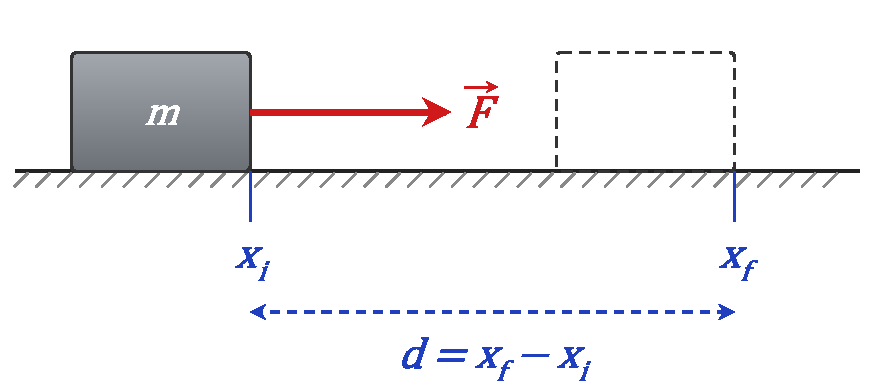
\includegraphics[width=0.7\textwidth]{Figuras_SVG_ENG/pdf/U4_trabajo_desplazamiento.pdf}
    \caption{Representation of Work}
    \label{fig:trabajo}
\end{figure}
When several forces act on the same body, the work done by those forces is the same as the work done by their resultant (the sum of ), that is:
\begin{centeredequation}
    \Sigma F = F_1 + F_2 + \dots
\end{centeredequation}
Therefore, the previous expression becomes:
\begin{centeredequation}
    W = \Sigma F \cdot d
    \label{eq:trabajo_2}
\end{centeredequation}
\begin{remark}
    Work is a form of energy, and therefore its SI unit is the joule.
\end{remark}

\begin{exercise}
    Calculate the work done by a donkey when it exerts a force of 2000 N on a cart and drags it for 400 meters.
    \begin{solu}
        The work is calculated using the formula:
        \[
            W = F \cdot d
        \]
        Where:
        \begin{itemize}
            \item $F = \qty{2000}{\newton}$ (force applied)
            \item $d = \qty{400}{\metre}$ (displacement)
        \end{itemize}
        Substituting the values:
        \[
            W = 2000 \times 400 = \qty{800000}{\joule} = \qty{800}{\kilo\joule}
        \]
        \textbf{Answer:} The donkey does \qty{800}{\kilo\joule} of work.
    \end{solu}
\end{exercise}

\begin{exercise}
    A student pushes a box with a force of 80 N and moves it \qty{5}{\metre} in the same direction as the force. Calculate the work done.
    \begin{solu}
        Using the work formula:
        \[
            W = F \cdot d = 80 \times 5 = \qty{400}{\joule}
        \]
        \textbf{Answer:} The work done is \qty{400}{\joule}.
    \end{solu}
\end{exercise}

\begin{exercise}
    A car is pushed by four people who exert a total force of \qty{600}{\newton}. If the car moves 8 meters, what work have they done?
    \begin{solu}

        \[
            W = F \cdot d = 600 \times 8 = \qty{4800}{\joule} = \qty{4.8}{\kilo\joule}
        \]
        \textbf{Answer:} They have done \qty{4.8}{\kilo\joule} of work.
    \end{solu}
\end{exercise}

\begin{exercise}
    A person drags a suitcase along the floor by applying a force of \qty{45}{\newton} over a displacement of \qty{25}{\metre}. Calculate the work done.
    \begin{solu}
        \[
            W = F \cdot d = 45 \times 25 = \qty{1125}{\joule} = \qty{1.125}{\kilo\joule}
        \]
        \textbf{Answer:} The work done is \qty{1.125}{\kilo\joule}.
    \end{solu}
\end{exercise}

\begin{exercise}
    Find the net work required to move a \qty{10}{\kilo\gram} block when the body moves 3 meters, with forces $F_1 = \qty{80}{\newton}$ and $F_2 = \qty{15}{\newton}$ acting in the same direction.
    \begin{solu}
        First, calculate the net force:
        \[
            F_{net} = F_1 + F_2 = 80 + 15 = \qty{95}{\newton}
        \]
        Then, calculate the work:
        \[
            W = F_{net} \cdot d = 95 \times 3 = \qty{285}{\joule}
        \]
        \textbf{Answer:} The net work is \qty{285}{\joule}.
    \end{solu}
\end{exercise}

\begin{exercise}
    A builder uses a pulley to lift a 50 kg mass to a height of 10 m. What work has been done? (Data: $g = \qty{9.8}{\mpss}$)
    \begin{solu}
        First, calculate the weight (force):
        \[
            F = m \cdot g = 50 \times 9.8 = \qty{490}{\newton}
        \]
        Then, calculate the work:
        \[
            W = F \cdot h = 490 \times 10 = \qty{4900}{\joule} = \qty{4.9}{\kilo\joule}
        \]
        \textbf{Answer:} The work done is \qty{4.9}{\kilo\joule}.
    \end{solu}
\end{exercise}


\section{Kinetic Energy}

Kinetic energy is the energy a body possesses when it is in motion.
The mathematical expression for kinetic energy is:

\vspace{12pt}
\begin{centeredequation}
    \eqnmarkbox[red]{energiacinetica}{E_k}
    =
    \dfrac{1}{2}
    \eqnmarkbox[blue]{masa}{m}
    \cdot
    \eqnmarkbox[mygreen]{velocidad}{v^2}
    \label{eq:energia_cinetica}
\end{centeredequation}
\annotate[yshift=1em]{left}{energiacinetica}{Kinetic Energy}
\annotate[yshift=1em]{}{masa}{mass}
\annotate[yshift=-1em]{below,left}{velocidad}{velocity}
\vspace{12pt}


\begin{exercise}
    A 1000 kg car travels at a speed of 20 m/s. Calculate its kinetic energy.
    \begin{solu}
        The kinetic energy formula is:
        \[
            E_k = \frac{1}{2}mv^2
        \]
        Where $m = \qty{1000}{\kilo\gram}$ and $v = \qty{20}{\mps}$:
        \[
            E_k = \frac{1}{2} \times 1000 \times 20^2 = \frac{1}{2} \times 1000 \times 400 = \qty{200000}{\joule} = \qty{200}{\kilo\joule}
        \]
        \textbf{Answer:} The kinetic energy is \qty{200}{\kilo\joule}.
    \end{solu}
\end{exercise}

\begin{exercise}
    A 0.5 kg ball moves with a speed of 10 m/s. What is its kinetic energy?
    \begin{solu}
        \[
            E_k = \frac{1}{2}mv^2 = \frac{1}{2} \times 0.5 \times 10^2 = 0.25 \times 100 = \qty{25}{\joule}
        \]
        \textbf{Answer:} The kinetic energy is \qty{25}{\joule}.
    \end{solu}
\end{exercise}

\begin{exercise}
    If a 4 kg object has a kinetic energy of 200 J, at what speed is it moving?
    \begin{solu}
        From $E_k = \frac{1}{2}mv^2$, we solve for $v$:
        \[
            v = \sqrt{\frac{2E_k}{m}} = \sqrt{\frac{2 \times 200}{4}} = \sqrt{\frac{400}{4}} = \sqrt{100} = \qty{10}{\mps}
        \]
        \textbf{Answer:} The object is moving at \qty{10}{\mps}.
    \end{solu}
\end{exercise}

\begin{exercise}
    What is the speed of an 80 kg athlete who has a kinetic energy of 8000 J?
    \begin{solu}
        \[
            v = \sqrt{\frac{2E_k}{m}} = \sqrt{\frac{2 \times 8000}{80}} = \sqrt{\frac{16000}{80}} = \sqrt{200} \approx \qty{14.14}{\mps}
        \]
        \textbf{Answer:} The athlete is moving at approximately \qty{14.14}{\mps}.
    \end{solu}
\end{exercise}


\section{Potential Energy}

We have two types of potential energy: gravitational potential energy and elastic potential energy.

\subsection{Gravitational Potential Energy}

This energy is a consequence of the position of a body (height).
The mathematical expression for potential energy is:

\vspace{6pt}
\begin{centeredequation}
    \eqnmarkbox[red]{energiapotencial}{E_p}
    =
    \eqnmarkbox[blue]{masa}{m}
    \cdot
    \eqnmarkbox[mygreen]{gravedad}{g}
    \cdot
    \eqnmarkbox[myOrange]{altura}{h}
    \label{eq:energia_potencial}
\end{centeredequation}
\annotate[yshift=1em]{left}{energiapotencial}{Potential Energy}
\annotate[yshift=1em]{}{masa}{mass}
\annotate[yshift=-1em]{below,left}{gravedad}{gravity}
\annotate[yshift=-1em]{below,right}{altura}{hight}
\vspace{12pt}


\begin{remark}
    Gravitational potential energy is commonly referred to simply as potential energy.
\end{remark}



\begin{exercise}
    A 2 kg book is on a shelf 1.5 m high. Calculate its gravitational potential energy. (Data: $g = 9.8$ m/s$^2$)
    \begin{solu}
        The gravitational potential energy formula is:
        \[
            E_p = mgh
        \]
        Where $m = \qty{2}{\kilo\gram}$, $g = \qty{9.8}{\mpss}$, and $h = \qty{1.5}{\metre}$:
        \[
            E_p = 2 \times 9.8 \times 1.5 = \qty{29.4}{\joule}
        \]
        \textbf{Answer:} The potential energy is \qty{29.4}{\joule}.
    \end{solu}
\end{exercise}

\begin{exercise}
    A 5 kg flowerpot is located on a balcony 12 m from the ground. What is its gravitational potential energy?
    \begin{solu}
        \[
            E_p = mgh = 5 \times 9.8 \times 12 = \qty{588}{\joule}
        \]
        \textbf{Answer:} The potential energy is \qty{588}{\joule}.
    \end{solu}
\end{exercise}

\begin{exercise}
    If an object has a potential energy of 600 J and is located 3 m high, what is its mass?
    \begin{solu}
        From $E_p = mgh$, we solve for $m$:
        \[
            m = \frac{E_p}{gh} = \frac{600}{9.8 \times 3} = \frac{600}{29.4} \approx \qty{20.41}{\kilo\gram}
        \]
        \textbf{Answer:} The mass is approximately \qty{20.41}{\kilo\gram}.
    \end{solu}
\end{exercise}

\begin{exercise}
    At what height must a 2 kilogram object be raised so that its potential energy is 125 J?
    \begin{solu}
        From $E_p = mgh$, we solve for $h$:
        \[
            h = \frac{E_p}{mg} = \frac{125}{2 \times 9.8} = \frac{125}{19.6} \approx \qty{6.38}{\metre}
        \]
        \textbf{Answer:} The object must be raised to approximately \qty{6.38}{\metre}.
    \end{solu}
\end{exercise}


\section{Mechanical Energy}

Mechanical energy is the sum of kinetic energy and potential energy.

\begin{centeredequation}
    E_m = E_k + E_p
    \label{eq:energia_mecanica}
\end{centeredequation}

\begin{exercise}
    Calculate the energy of the following objects:
    \begin{enumerate}[label=\alph*)]
\item A 1200 kg car travelling at a speed of \qty{6}{\mps}
\item A 450 gram picture frame located 1.75 meters above the ground.
\item A 60 gram tennis ball with a speed of \qty{65}{\mps} and a height of 1.25 meters.
    \end{enumerate}
    \begin{solu}
        a) Kinetic energy only:
        \[
            E_k = \frac{1}{2} \times 1200 \times 6^2 = \frac{1}{2} \times 1200 \times 36 = \qty{21600}{\joule} = \qty{21.6}{\kilo\joule}
        \]
        b) Potential energy only (convert to kg: 450 g = 0.45 kg):
        \[
            E_p = 0.45 \times 9.8 \times 1.75 = \qty{7.72}{\joule}
        \]
        c) Both kinetic and potential (convert to kg: 60 g = 0.06 kg):
        \[
            E_k = \frac{1}{2} \times 0.06 \times 65^2 = \frac{1}{2} \times 0.06 \times 4225 = \qty{126.75}{\joule}
        \]
        \[
            E_p = 0.06 \times 9.8 \times 1.25 = \qty{0.735}{\joule}
        \]
        \[
            E_M = E_k + E_p = 126.75 + 0.735 = \qty{127.49}{\joule}
        \]
        \textbf{Answers:} a) \qty{21.6}{\kilo\joule}, b) \qty{7.72}{\joule}, c) \qty{127.49}{\joule}
    \end{solu}
\end{exercise}

\begin{exercise}
    Find the mechanical energy of an eagle of 2500 grams that is flying at a speed of \qty{100}{\kmph} and at a height of 250 m.
    \begin{solu}
        First, convert units:
        \begin{itemize}
            \item Mass: 2500 g = 2.5 kg
            \item Speed: 100 km/h = $\frac{100 \times 1000}{3600} = \qty{27.78}{\mps}$
        \end{itemize}
        Calculate kinetic energy:
        \[
            E_k = \frac{1}{2} \times 2.5 \times 27.78^2 = \frac{1}{2} \times 2.5 \times 771.73 = \qty{964.66}{\joule}
        \]

        Calculate potential energy:
        \[
            E_p = 2.5 \times 9.8 \times 250 = \qty{6125}{\joule}
        \]

        Total mechanical energy:
        \[
            E_M = E_k + E_p = 964.66 + 6125 = \qty{7089.66}{\joule} \approx \qty{7.09}{\kilo\joule}
        \]
        \textbf{Answer:} The mechanical energy is approximately \qty{7.09}{\kilo\joule}.
    \end{solu}
\end{exercise}

\begin{exercise}
    Of the following situations, which will have the greatest mechanical energy?:
    \begin{enumerate}[label=\alph*)]
\item A 10 kg rock at a height of 5 meters.
\item A 5 kg rock at a height of 10 meters.
\item A 250-gram drone flying close to the ground at a speed of \qty{25}{\mps}
\item A 500-gram stone at a height of 250 meters and a speed of \qty{10}{\mps}
    \end{enumerate}
    \begin{solu}
        a) $E_p = 10 \times 9.8 \times 5 = \qty{490}{\joule}$

        b) $E_p = 5 \times 9.8 \times 10 = \qty{490}{\joule}$

        c) $E_k = \frac{1}{2} \times 0.25 \times 25^2 = \frac{1}{2} \times 0.25 \times 625 = \qty{78.13}{\joule}$

        d) $E_k = \frac{1}{2} \times 0.5 \times 10^2 = 25$ J; $E_p = 0.5 \times 9.8 \times 250 = 1225$ J; $E_M = \qty{1250}{\joule}$

        \textbf{Answer:} Option d) has the greatest mechanical energy with \qty{1250}{\joule}.
    \end{solu}
\end{exercise}

\begin{exercise}
    A 0.4 kg ball is at a height of 5 m and moves with a speed of 8 m/s. Calculate:
    \begin{enumerate}
        \item Its potential energy
        \item Its kinetic energy
        \item Its total mechanical energy
    \end{enumerate}
    \begin{solu}
        1. Potential energy:
        \[
            E_p = 0.4 \times 9.8 \times 5 = \qty{19.6}{\joule}
        \]
        2. Kinetic energy:
        \[
            E_k = \frac{1}{2} \times 0.4 \times 8^2 = 0.2 \times 64 = \qty{12.8}{\joule}
        \]
        3. Total mechanical energy:
        \[
            E_M = E_p + E_k = 19.6 + 12.8 = \qty{32.4}{\joule}
        \]
        \textbf{Answers:} 1) \qty{19.6}{\joule}, 2) \qty{12.8}{\joule}, 3) \qty{32.4}{\joule}
    \end{solu}
\end{exercise}

\begin{exercise}
    A 0.2 kg bird flies at a height of 15 m with a speed of 12 m/s. Determine its total mechanical energy.
    \begin{solu}
        Kinetic energy:
        \[
            E_k = \frac{1}{2} \times 0.2 \times 12^2 = 0.1 \times 144 = \qty{14.4}{\joule}
        \]
        Potential energy:
        \[
            E_p = 0.2 \times 9.8 \times 15 = \qty{29.4}{\joule}
        \]
        Total mechanical energy:
        \[
            E_M = 14.4 + 29.4 = \qty{43.8}{\joule}
        \]
        \textbf{Answer:} The total mechanical energy is \qty{43.8}{\joule}.
    \end{solu}
\end{exercise}


\section{Principle of Conservation of Mechanical Energy}


\begin{dBox}
    \textbf{The principle of conservation of mechanical energy states say}: mechanical energy at the beginning (we set an initial point, represented in the formula with \( i \)) will be equal to mechanical energy at the end (we set the final point, represented in the formula with \( f \))
\end{dBox}

Mathematically, this principle can be expressed as:
\begin{centeredequation}
    E_{m,i} = E_{m,f}
    \label{eq:conservacion_energia}
\end{centeredequation}
This expression can also be written as:
\begin{centeredequation}
    E_{p,i} + E_{c,i}  = E_{p,f} + E_{c,f}
    \label{eq:conservacion_energia_semidesarrollada}
\end{centeredequation}
If we develop this expression further, we get:
\begin{centeredequation}
    m\cdot g \cdot h_i + \dfrac{1}{2} \cdot m\ v_i^2 = m\cdot g \cdot h_f + \dfrac{1}{2} \cdot m\ v_f^2
    \label{eq:conservacion_energia_desarrollada}
\end{centeredequation}

\begin{exercise}
    A 50 kg metal sphere is dropped from a height of 8 meters to the ground.
    \begin{enumerate}[label=\alph*)]
\item Calculate the mechanical energy it has at the moment it is dropped.
\item With what speed does it reach the ground?
    \end{enumerate}
    \begin{solu}
        a) At the moment of release, all energy is potential:
        \[
            E_M = E_p = mgh = 50 \times 9.8 \times 8 = \qty{3920}{\joule}
        \]
        b) By conservation of energy, at ground level all energy is kinetic:
        \[
            E_k = E_M \Rightarrow \frac{1}{2}mv^2 = 3920
        \]
        \[
            v = \sqrt{\frac{2 \times 3920}{50}} = \sqrt{\frac{7840}{50}} = \sqrt{156.8} \approx \qty{12.52}{\mps}
        \]
        Alternatively: $v = \sqrt{2gh} = \sqrt{2 \times 9.8 \times 8} = \sqrt{156.8} \approx \qty{12.52}{\mps}$
        \textbf{Answers:} a) \qty{3920}{\joule}, b) \qty{12.52}{\mps}
    \end{solu}
\end{exercise}

\begin{exercise}
    From a height of \qty{15}{\metre}, an object of mass \qty{3}{\kilo\gram} is thrown vertically downward with an initial speed of \qty{2}{\mps}. If there is no air resistance, find:
    \begin{enumerate}[label=\alph*)]
\item The kinetic energy at 5 meters above the ground.
\item The speed at that moment and the speed with which it reaches the ground.
    \end{enumerate}
    \begin{solu}
        Initial energy (at h = 15 m):
        \[
            E_k = \frac{1}{2} \times 3 \times 2^2 = \qty{6}{\joule}
        \]
        \[
            E_p = 3 \times 9.8 \times 15 = \qty{441}{\joule}
        \]
        \[
            E_{M,initial} = 6 + 441 = \qty{447}{\joule}
        \]
        a) At h = 5 m:
        \[
            E_p = 3 \times 9.8 \times 5 = \qty{147}{\joule}
        \]
        \[
            E_k = E_M - E_p = 447 - 147 = \qty{300}{\joule}
        \]
        b) Speed at h = 5 m:
        \[
            v = \sqrt{\frac{2E_k}{m}} = \sqrt{\frac{2 \times 300}{3}} = \sqrt{200} \approx \qty{14.14}{\mps}
        \]
        Speed at ground (h = 0):
        \[
            E_k = E_M = 447 \text{ J}
        \]
        \[
            v = \sqrt{\frac{2 \times 447}{3}} = \sqrt{298} \approx \qty{17.26}{\mps}
        \]
        \textbf{Answers:} a) \qty{300}{\joule}, b) \qty{14.14}{\mps} at 5 m height, \qty{17.26}{\mps} at ground
    \end{solu}
\end{exercise}

\begin{exercise}
    On a slide 2 meters high, there is a 25 kg child. With what speed would they reach the ground when sliding down?
    \begin{solu}
        By conservation of energy:
        \[
            E_{p,initial} = E_{k,final}
        \]
        \[
            mgh = \frac{1}{2}mv^2
        \]
        \[
            v = \sqrt{2gh} = \sqrt{2 \times 9.8 \times 2} = \sqrt{39.2} \approx \qty{6.26}{\mps}
        \]
        \textbf{Answer:} The child reaches the ground at approximately \qty{6.26}{\mps}.
    \end{solu}
\end{exercise}

\begin{exercise}
    A 0.5 kg ball is dropped from a window 30 m above the street. Calculate:
    \begin{enumerate}[label=\alph*)]
\item The potential energy relative to the ground at the moment of release.
\item The kinetic energy at the moment it reaches the ground.
\item The speed with which it hits the ground.
    \end{enumerate}
    \begin{solu}
        a) Potential energy at release:
        \[
            E_p = 0.5 \times 9.8 \times 30 = \qty{147}{\joule}
        \]
        b) By conservation of energy, all potential energy converts to kinetic:
        \[
            E_k = \qty{147}{\joule}
        \]
        c) Speed at ground:
        \[
            v = \sqrt{2gh} = \sqrt{2 \times 9.8 \times 30} = \sqrt{588} \approx \qty{24.25}{\mps}
        \]
        \textbf{Answers:} a) \qty{147}{\joule}, b) \qty{147}{\joule}, c) \qty{24.25}{\mps}
    \end{solu}
\end{exercise}

\begin{exercise}
    At the top of a roller coaster, a car and its occupants with a total mass of 1000 kg are at a height of 50 meters above the ground and have a speed of \qty{5}{\mps}.
    \begin{enumerate}[label=\alph*)]
\item What speed will the car have when it reaches the next hilltop, which is at a height of 25 meters above the ground?
\item If the speed it has at the next hilltop is \qty{20}{\mps}, what is the work done by friction between the wheels and the rails?
    \end{enumerate}
    \begin{solu}
        Initial energy (\( h_1 = \qty{50}{\metre} \), \( v_1 = \qty{5}{\metre\per\second} \)):
        \[
            E_{M1} = \frac{1}{2} \times 1000 \times 5^2 + 1000 \times 9.8 \times 50 = 12500 + 490000 = \qty{502500}{\joule}
        \]
        a) Without friction, at \( h_2 = \qty{25}{\metre} \):
        \[
            E_p = 1000 \times 9.8 \times 25 = \qty{245000}{\joule}
        \]
        \[
            E_k = E_{M1} - E_p = 502500 - 245000 = \qty{257500}{\joule}
        \]
        \[
            v = \sqrt{\frac{2 \times 257500}{1000}} = \sqrt{515} \approx \qty{22.69}{\mps}
        \]
        b) Actual energy at \( h_2 \) with \( v_2 \) = \qty{20}{\metre\per\second}:
        \[
            E_{M2} = \frac{1}{2} \times 1000 \times 20^2 + 245000 = 200000 + 245000 = \qty{445000}{\joule}
        \]
        Work done by friction (negative because it opposes motion):
        \[
            W_{friction} = E_{M2} - E_{M1} = 445000 - 502500 = \qty{-57500}{\joule}
        \]
        \textbf{Answers:} a) \qty{22.69}{\mps}, b) \qty{-57500}{\joule} (or \qty{57500}{\joule} of energy lost)
    \end{solu}
\end{exercise}

\begin{exercise}
    A 0.3 kg ball is dropped from a height of 10 m. Calculate:
    \begin{enumerate}
        \item The initial mechanical energy
        \item The speed with which it reaches the ground
        \item The kinetic energy just before touching the ground
    \end{enumerate}
    \begin{solu}
        1. Initial mechanical energy (all potential):
        \[
            E_M = mgh = 0.3 \times 9.8 \times 10 = \qty{29.4}{\joule}
        \]
        2. Speed at ground:
        \[
            v = \sqrt{2gh} = \sqrt{2 \times 9.8 \times 10} = \sqrt{196} = \qty{14}{\mps}
        \]
        3. Kinetic energy at ground (equals initial mechanical energy):
        \[
            E_k = \qty{29.4}{\joule}
        \]
        \textbf{Answers:} 1) \qty{29.4}{\joule}, 2) \qty{14}{\mps}, 3) \qty{29.4}{\joule}
    \end{solu}
\end{exercise}

\begin{exercise}
    A pendulum has a mass of 0.5 kg and is released from a height of 2 m. If there is no friction:
    \begin{enumerate}
        \item What is its initial potential energy?
        \item What will be its maximum speed at the lowest point?
        \item What kinetic energy will it have when it is at a height of 1 m?
    \end{enumerate}
    \begin{solu}
        1. Initial potential energy:
        \[
            E_p = 0.5 \times 9.8 \times 2 = \qty{9.8}{\joule}
        \]
        2. Maximum speed at lowest point (h = 0):
        \[
            v = \sqrt{2gh} = \sqrt{2 \times 9.8 \times 2} = \sqrt{39.2} \approx \qty{6.26}{\mps}
        \]
        3. At h = 1 m:
        \[
            E_p = 0.5 \times 9.8 \times 1 = \qty{4.9}{\joule}
        \]
        \[
            E_k = E_M - E_p = 9.8 - 4.9 = \qty{4.9}{\joule}
        \]
        \textbf{Answers:} 1) \qty{9.8}{\joule}, 2) \qty{6.26}{\mps}, 3) \qty{4.9}{\joule}
    \end{solu}
\end{exercise}

\begin{exercise}
    A 70 kg skier starts from rest from the top of a slope located 20 m high. If we neglect friction, with what speed will they reach the base of the slope?
    \begin{solu}
        Using conservation of energy:
        \[
            v = \sqrt{2gh} = \sqrt{2 \times 9.8 \times 20} = \sqrt{392} \approx \qty{19.80}{\mps}
        \]
        \textbf{Answer:} The skier will reach the base at approximately \qty{19.80}{\mps}.
    \end{solu}
\end{exercise}


\section{Power}

Another important quantity is power (\( P \)). Power can be defined as the energy (\( E \)) or work (\( W \)) done per unit of time (\( t \)), and its mathematical expression is:
\begin{centeredequation}
    P = \dfrac{E}{t}
    \label{eq:potencia_energia}
\end{centeredequation}
or equivalently:
\begin{centeredequation}
    P = \dfrac{W}{t}
    \label{eq:potencia_trabajo}
\end{centeredequation}

The unit of power in the SI system is the Watt (\unit{\watt}). Another widely used unit of power is the horsepower (HP), where
\( 1\ HP = \qty{735}{\watt} \)

\begin{exercise}
    A crane lifts a load of $500\,\text{kg}$ to a height of $20\,\text{meters}$ in $10\,\text{seconds}$. Calculate the power developed by the crane. (Use $g = 9.8\,\text{m/s}^2$).
    \begin{solu}
        First, we calculate the work done (potential energy): $W = m \cdot g \cdot h$ \\
        $W = 500\,\text{kg} \cdot 9.8\,\text{m/s}^2 \cdot 20\,\text{m} = 98,000\,\text{J}$ \\
        Now, we find the power: $P = \frac{W}{t} = \frac{98,000\,\text{J}}{10\,\text{s}} = \mathbf{9800\,\text{W}}$
    \end{solu}
\end{exercise}

\begin{exercise}
    An electric motor has a power of $1200\,\text{W}$. How long will it take to perform $18,000\,\text{J}$ of work?
    \begin{solu}
        Using the formula $P = \frac{W}{t}$, we rearrange to solve for $t$: \\
        $t = \frac{W}{P} = \frac{18,000\,\text{J}}{1200\,\text{W}} = \mathbf{15\,\text{seconds}}$
    \end{solu}
\end{exercise}

\begin{exercise}
    A student with a mass of $60\,\text{kg}$ climbs a staircase $5\,\text{meters}$ high in $12\,\text{seconds}$.
    Calculate the power generated.
    \begin{solu}
        $W = m \cdot g \cdot h = 60\,\text{kg} \cdot 9.8\,\text{m/s}^2 \cdot 5\,\text{m} = 2940\,\text{J}$ \\
        $P = \frac{2940\,\text{J}}{12\,\text{s}} = \mathbf{245\,\text{W}}$
    \end{solu}
\end{exercise}

\begin{exercise}
    A light bulb has a power of $60\,\text{W}$.
    If it remains on for $2\,\text{hours}$, how much total energy (in Joules) does it consume?
    \begin{solu}
        First, convert time to seconds: $2\,\text{h} \cdot 3600\,\text{s/h} = 7200\,\text{s}$ \\
        $E = P \cdot t = 60\,\text{W} \cdot 7200\,\text{s} = \mathbf{432,000\,\text{J}}$ (or $4.32 \cdot 10^5\,\text{J}$)
    \end{solu}
\end{exercise}


\section{Domestic Energy Consumption}

Figure \ref{fig:factura_luz} shows the information usually found in an electricity bill.

\begin{figure}[H]
    \centering
%    \includegraphics[scale=0.9]{images/energia/factura_luz}
    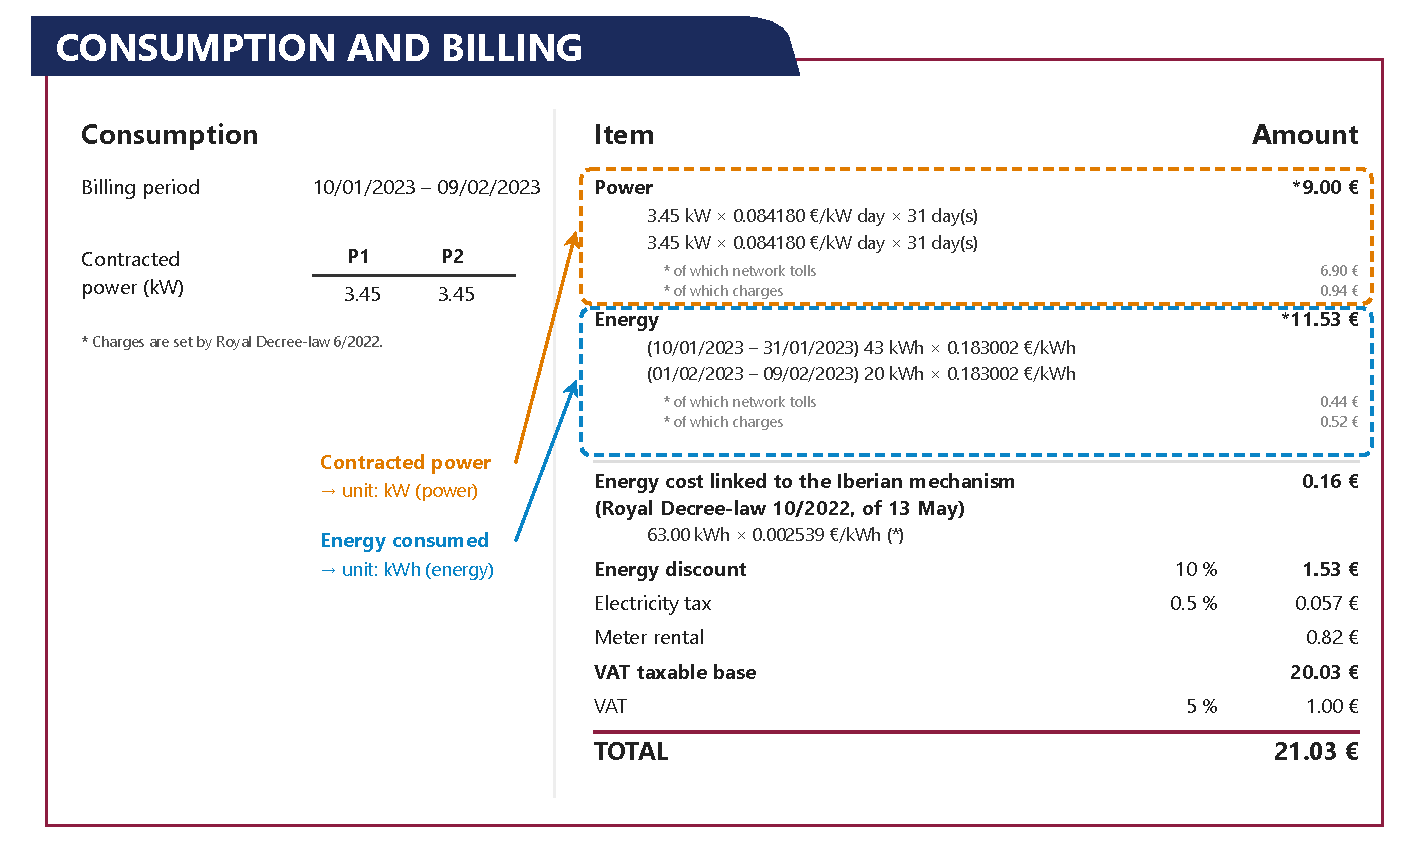
\includegraphics[width=\textwidth]{Figuras_SVG_ENG/pdf/U4_factura_luz.pdf}
    \caption{Information Found on an Electricity Bill}
    \label{fig:factura_luz}
\end{figure}

First, we see that we must pay for the contracted power.
As we have seen, power is the energy per unit of time supplied, and its SI unit is the watt (\unit{\watt}).

In this case, the contracted power is \qty{3.45}{\kilo\watt}.
F
\begin{remark}
    Here we see a unit conversion using conversion factors to calculate the price we must pay after 31 days for the contracted power.
\end{remark}
\begin{example}
    Calculate the price we have to pay for 31 days using conversion factors. Next, it shows the energy consumed as well as the price to pay.
    In this case, it is \( 0.084180 \dfrac{\text{€}}{\unit{\kwh}} \) and we see that \qty{43}{\kwh} was consumed first, followed by \qty{20}{\kwh}.
\end{example}


\begin{remark}
    It is important not to confuse \unit{\kwh}, which is a unit of energy, with \unit{\watt}, which is a unit of power.\\
    Calculate the equivalence between \unit{\kwh} and joules.
\end{remark}

\begin{exercise}
    You should review a home electricity bill and calculate the cost of having three appliances switched on for a certain period of time.
\end{exercise}


\section{Energy Sources}

An \textbf{energy source} is a natural resource from which energy can be obtained and transformed into other forms.
According to their regeneration capacity, we have:

\begin{enumerate}[label=\numberballmDarkTeal]
\item \negsubro{Renewable}.
The regeneration rate equals the consumption rate, and they can be considered inexhaustible.
\begin{itemize}
    \item Hydroelectric energy.
    \item Solar energy.
    \item Geothermal energy.
    \item Biomass.
    \item Marine energy.
    \item Wind energy.
\end{itemize}
\item \negsubro{Non-renewable}
\end{enumerate}


\section{Heat and Temperature}

Often, the terms heat and temperature are confused.

\textbf{Heat} is the amount of energy transferred from one body to another due to a temperature difference.
For heat to exist, two bodies must be in contact.
Since heat is a form of energy, its SI unit is the joule.

\textbf{Temperature} is the measure of the kinetic energy of the molecules of a substance.
The SI unit is the Kelvin, although degrees Celsius are widely used.

\begin{centeredequation}
    \unit{\kelvin} = \unit{\degreeCelsius} + 273
\end{centeredequation}
\begin{centeredequation}
    \unit{\degreeCelsius} = \unit{\kelvin} - 273
\end{centeredequation}

\begin{remark}
    We can say that the temperature is very high but the heat is low.\\
    Could you explain why?
\end{remark}

\begin{exercise}
    Explain why the temperature on the surface of the sun is very high, while its heat is not as high in comparison.
    Find the answer online, including relevant sources.
\end{exercise}

\section{Vocabulary}


\begin{vocabulary}[Energy]
The capacity to do work or produce change in a physical system. \newline
\textbf{Translation to Spanish}: Energía \newline
% Line 10
\end{vocabulary}


\begin{vocabulary}[Kinetic Energy]
The energy possessed by an object due to its motion. \newline
\textbf{Translation to Spanish}: Energía cinética \newline
% Line 52
\end{vocabulary}


\begin{vocabulary}[Potential Energy]
Stored energy associated with the position or configuration of an object. \newline
\textbf{Translation to Spanish}: Energía potencial \newline
% Line 73
\end{vocabulary}


\begin{vocabulary}[Mechanical Energy]
The sum of kinetic and potential energy in a system. \newline
\textbf{Translation to Spanish}: Energía mecánica \newline
% Line 89
\end{vocabulary}


\begin{vocabulary}[Work]
The transfer of energy that occurs when a force moves an object through a distance. \newline
\textbf{Translation to Spanish}: Trabajo \newline
% Line 132
\end{vocabulary}


\begin{vocabulary}[Power]
The rate at which work is done or energy is transferred. \newline
\textbf{Translation to Spanish}: Potencia \newline
% Line 174
\end{vocabulary}


\begin{vocabulary}[Conservation of Energy]
A principle stating that energy cannot be created or destroyed, only transformed from one form to another. \newline
\textbf{Translation to Spanish}: Conservación de la energía \newline
% Line 214
\end{vocabulary}


\begin{vocabulary}[Thermal Energy]
The internal energy of a system associated with the random motion of its particles. \newline
\textbf{Translation to Spanish}: Energía térmica \newline
% Line 247
\end{vocabulary}


\begin{vocabulary}[Heat]
The transfer of thermal energy between systems due to a temperature difference. \newline
\textbf{Translation to Spanish}: Calor \newline
% Line 281
\end{vocabulary}


\begin{vocabulary}[Temperature]
A measure of the average kinetic energy of the particles in a substance. \newline
\textbf{Translation to Spanish}: Temperatura \newline
% Line 298
\end{vocabulary}

